\section{Introduction}

This sprint focuses on the authentication layer of the HexStrike platform and on the access control rules that protect the main application modules. The goal of this iteration is to provide a secure entry point to the system, manage user sessions with JWT, and restrict sensitive actions such as scan creation and scan history access to authenticated users only.

In practice, this sprint covers the login and registration flow, the guest session mechanism, protected routes on the frontend, and the backend middleware that validates every secured request.

\subsection{Sprint Purpose}

The purpose of this sprint is to secure the platform's entry points and session management to enable safe use of the scanning and analysis features. Concretely, the sprint delivers a robust authentication system, a guest mode for quick evaluation, and middleware that enforces access control for all sensitive API endpoints.

\section{Sprint Backlog}

The backlog of this sprint contains the following user stories:

\begin{table}[H]
    \centering
    \renewcommand{\arraystretch}{1.2}
    \begin{tabularx}{\textwidth}{|X|}
        \hline
        As a visitor, I can create an account and log in to the platform. \\\hline
        As a user, I can start a temporary guest session without creating a persistent account. \\\hline
        As an authenticated user, I can access protected pages such as the scanner and scan history. \\\hline
        As a guest user, I cannot access protected resources or save scans in the database. \\\hline
        As the system, I can verify and refresh the current session by exposing the authenticated user profile. \\\hline
    \end{tabularx}
    \caption{Sprint Backlog}
\end{table}

\section{Requirements Analysis}

\subsection{Use Case Diagram}

The actors involved in this sprint are the visitor, the registered user, and the guest user. The visitor can register and log in, the registered user can access protected modules, and the guest user can only use limited temporary access.

The following figure is reserved for the use case diagram of this sprint.

\begin{figure}[H]
    \centering
    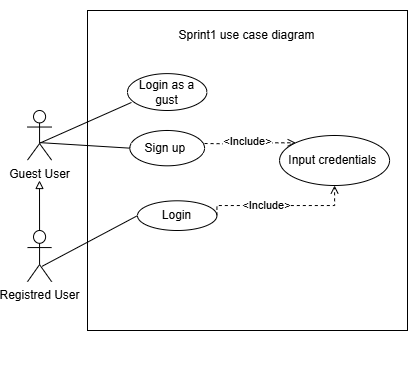
\includegraphics[width=0.85\textwidth]{uploads/diagrams/sprint1usecase.drawio.png}
    \caption{Use case diagram for authentication and access control}
    \label{fig:sprint1-usecase}
\end{figure}

\subsection{Use Case Description}

The main use cases of this sprint are summarized in the following tables.

\begin{table}[H]
    \centering
    \renewcommand{\arraystretch}{1.2}
    \begin{tabular}{|p{3cm}|p{11cm}|}
        \hline
        \textbf{Use case} & Register \\ \hline
        \textbf{Actor} & Visitor \\ \hline
        \textbf{Description} & The visitor creates a new account by providing a full name, an email address, and a password. The backend validates the input, hashes the password, stores the user in the database, and returns a JWT token. \\ \hline
        \textbf{Pre-condition} & The visitor does not already have an active authenticated session. \\ \hline
        \textbf{Post-condition} & The user account is created and the session becomes authenticated. \\ \hline
    \end{tabular}
    \caption{Use case description: Register}
    \label{tab:register-usecase}
\end{table}

\begin{table}[H]
    \centering
    \renewcommand{\arraystretch}{1.2}
    \begin{tabular}{|p{3cm}|p{11cm}|}
        \hline
        \textbf{Use case} & Login \\ \hline
        \textbf{Actor} & User \\ \hline
        \textbf{Description} & The user provides valid credentials. The backend checks the password, generates a signed JWT token, and returns the authenticated profile. \\ \hline
        \textbf{Pre-condition} & The user account already exists in the database. \\ \hline
        \textbf{Post-condition} & The user is authenticated and can access protected pages. \\ \hline
    \end{tabular}
    \caption{Use case description: Login}
    \label{tab:login-usecase}
\end{table}

\begin{table}[H]
    \centering
    \renewcommand{\arraystretch}{1.2}
    \begin{tabular}{|p{3cm}|p{11cm}|}
        \hline
        \textbf{Use case} & Guest login \\ \hline
        \textbf{Actor} & Visitor \\ \hline
        \textbf{Description} & The system creates a temporary guest session for quick access. This session is limited and does not allow scan persistence or access to scan history. \\ \hline
        \textbf{Pre-condition} & The user is not connected with a registered account. \\ \hline
        \textbf{Post-condition} & A temporary guest token is created and stored on the client side. \\ \hline
    \end{tabular}
    \caption{Use case description: Guest login}
    \label{tab:guest-usecase}
\end{table}

\section{Design}

\subsection{Class Diagram}

The design of this sprint is based on the separation between frontend and backend responsibilities.

On the backend side, the authentication flow is handled by the Auth controller and service, the user data is stored in the Prisma User model, and the secured routes are protected by the authentication middleware. The server also applies rate limiting to login endpoints to reduce brute-force attempts.

On the frontend side, the AuthContext manages the session state, the Login and Register pages collect credentials, and the ProtectedRoute and PublicOnlyRoute components control access to the application pages.

The following figure is reserved for the refined class diagram of this sprint.

\begin{figure}[H]
    \centering
    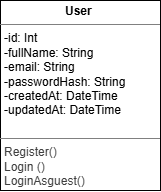
\includegraphics[width=0.3\textwidth]{uploads/diagrams/sprint1classediagram.drawio.png}
    \caption{Class diagram for Sprint 1}
    \label{fig:sprint3-class-diagram}
\end{figure}

\subsection{Sequence Diagram}

The main sequence of this sprint starts when the user submits login credentials from the frontend. The frontend sends the request to the backend, the backend verifies the credentials, and if they are valid, a JWT token is returned and stored locally by the client.

After authentication, every protected request includes the token in the authorization header. The backend middleware checks the token before allowing access to scan creation, scan history, and detailed scan reports. Guest sessions follow the same flow, but the backend blocks access to privileged operations.

The following figure is reserved for the sequence diagram of this sprint.

\begin{figure}[H]
    \centering
    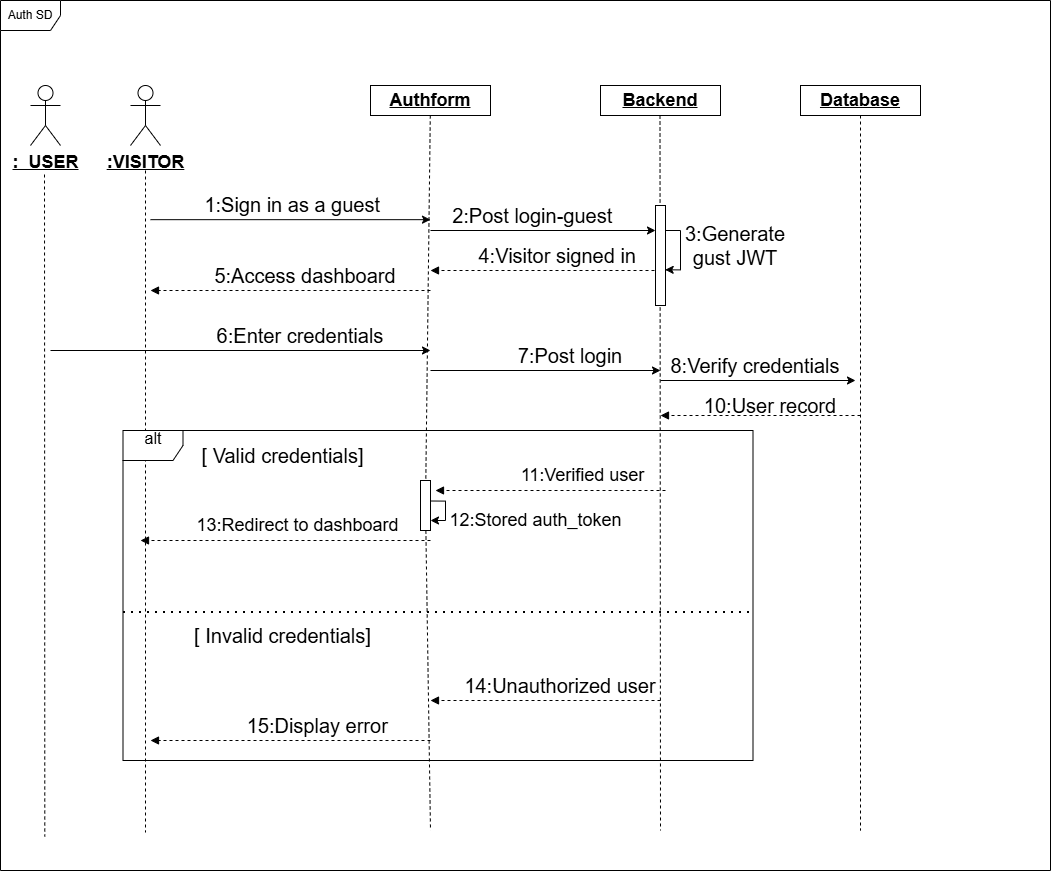
\includegraphics[width=0.98\textwidth]{uploads/diagrams/sprint 1 sequence.drawio.png}
    \caption{Sequence diagram for authentication and access control}
    \label{fig:sprint1-sequence-diagram}
\end{figure}

\section{Implementation}

In this sprint, we present the interfaces developed for Sprint 1. The implementation includes authentication pages (login and registration). The following figures illustrate the application interfaces:

\begin{figure}[H]
    \centering
    \fbox{\parbox{0.85\textwidth}{\centering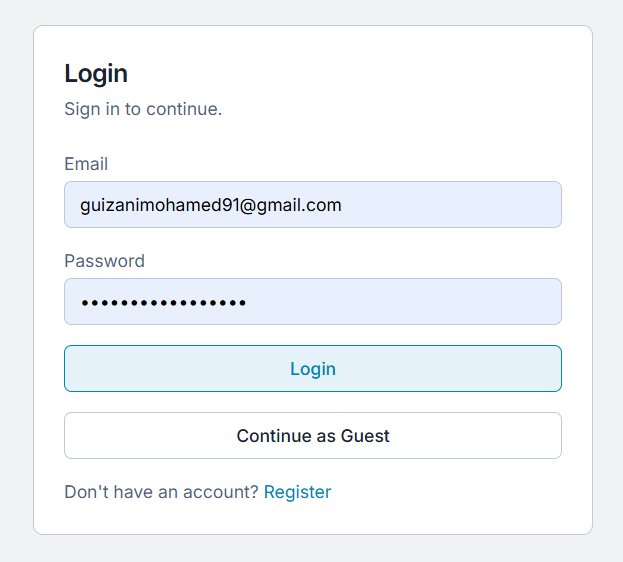
\includegraphics[width=0.85\textwidth]{uploads/images/login.png}}}%
    \caption{Login page}
    \label{fig:login-page}
\end{figure}

\begin{figure}[H]
    \centering
    \fbox{\parbox{0.85\textwidth}{\centering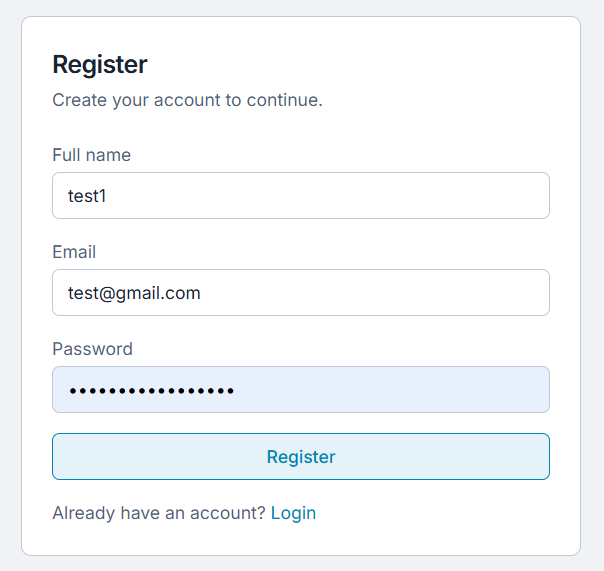
\includegraphics[width=0.85\textwidth]{uploads/images/sign up.png}}}%
    \caption{sign up  page}
    \label{fig:sizgn-up-page}
\end{figure}




 

\section{Conclusion}

This sprint established the authentication and access control layer of the HexStrike platform. It provided a secure login flow, a temporary guest mode, and protected access to sensitive pages and API endpoints.

The next sprint can now focus on the scanning workflow, vulnerability processing, and reporting features on top of this secured foundation.